% LaTeX Report Template - customizing page format
%
% LaTeX document uses 10-point fonts by default.  To use
% 11-point or 12-point fonts, use \documentclass[11pt]{report}
% or \documentclass[12pt]{report}.
\documentclass{report}
\usepacakage[margin=lin]{geometetry}
\usepackackage{graphicx}

% Set left margin - The default is 1 inch, so the following 
% command sets a 1.25-inch left margin.
\setlength{\oddsidemargin}{0.25in}

% Set width of the text - What is left will be the right margin.
% In this case, right margin is 8.5in - 1.25in - 6in = 1.25in.
\setlength{\textwidth}{6in}

% Set top margin - The default is 1 inch, so the following 
% command sets a 0.75-inch top margin.
\setlength{\topmargin}{-0.25in}

% Set height of the text - What is left will be the bottom margin.
% In this case, bottom margin is 11in - 0.75in - 9.5in = 0.75in
\setlength{\textheight}{8in}

% Set the beginning of a LaTeX document
\begin{document}
\begin{titlepage}
    \begin{center}
\line(1,0){500}\\
\huge{\bfseries A REPORT ABOUT SPORTS PARTICIPATION IN MAKERERE\\}
\line(1,0){500}\\
[0.25in]
\huge{\bfseries A REPORT SUBMITTED TO THE SCHOOL OF COMPUTING AND INFORMATICS TECHNOLOGY}\\ 
[1.5in] 
\line(1,0){300}\\ 
\huge{\bfseries MY DETAILS}
\line(1,0){300}\\ 
Kuzanya John Bosco	|14/U/8343/ps	|214014659\\
    \end{center}
\end{titlepage} 
       

\section{Introduction}   
Regular physical activity confers multiple physical and mental health benefits and plays a vital role in efforts to combat childhood obesity.
The U.S. Department of Health and Human Services suggests that children and adolescents accumulate 60 minutes of physical activity every day,yet
most young people do not meet these guidelines. Further,physical activity levels tend to decline during adolescence suggesting that efforts to promote physical activity during this period are essential.Participation in organized university sports offers opportunities for students of all ages to be physically active and has been shown to help improve students� self-esteem and psychological well-being. While participation in sports can
play an important role in increasing physical activity levels,as some have noted, sports participation alone may not be sufficient to meet the current physical activity recommendations for adolescents.9 Therefore sports participation should not be seen as a replacement for physical education in schools but rather as a supplement to the solid foundation provided by physical education. 
   
\section{Background to the problem.}  
The findings in this brief are based on data from the Bridging the Gap study. More than 2,000 surveys were completed by administrators (mostly principals) of 8th,10th and 12th grade students in public universities across three  years,2008�2009, 2009�2010 and 2010�2011. The resulting data are weighted such that the results are representative of students in public schools in the coterminous U.S. at each grade level. Schools were categorized as low-, mid-, or highSES based on the percentage of students who were eligible for a free or reduced-price lunch. university were categorized as having a low, moderate or high number of sports facilities based on the availability of  different facilities.
The relationships between university socio-economic level, availability of facilities and gender with sports participation (i.e., participation in interscholastic sports and intramural sports, separately) were tested using multivariate regression models that controlled for the number of students in the university and time of data collection
\section{Key Findings}
The percentage of students participating in interscholastic sports during the university year is relatively consistent across
Higher percentages of boys than girls participate in interscholastic sports and intramural sports. The gender gap is between 2 percent to 5 percent, which is statistically significant and present for all grades. 
Student participation in interscholastic sports is higher at
universities with more sports facilities compared with schools that have few facilities . This relationship remains even after considering university.
The percentage of students participating in intramural sports does not vary with the number of sports facilities.
\section{Main Objective}
To develop a high-performance computing system that can do automatic collection of data about student's sports participation in universities.
\subsection{Specific Objectives}
To collect and analyze the requirements about the relevance and feasibility of the Automatic collection of data about student's sports participation in universities.\\ 
To implement the data collection application.\\
To test and validate the application.\\

\section{Research Scope}
This research is based on Efficient sport participation by the students on the uniiversity.
\section{Methodology}
\subsection{physical Contact}
Through this i was able to collect data from different students while performing their specific sports in their free time
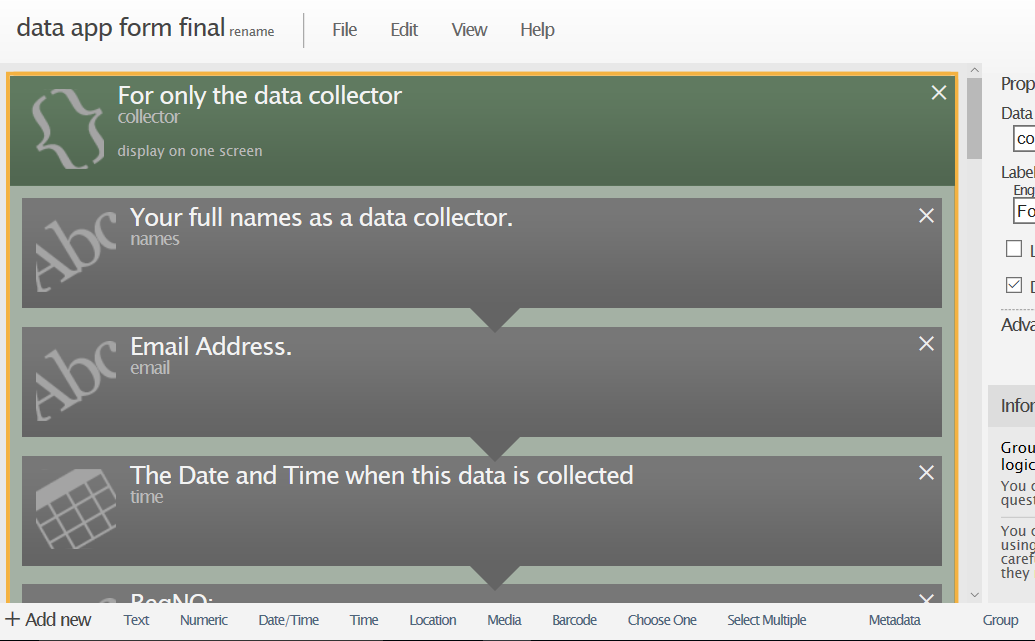
\includegraphics[width=6cm,height=8cm]{Capture}
\subsection{Questionaires}
while using ODK collect as a tool,i was able to design a questionair form as below.
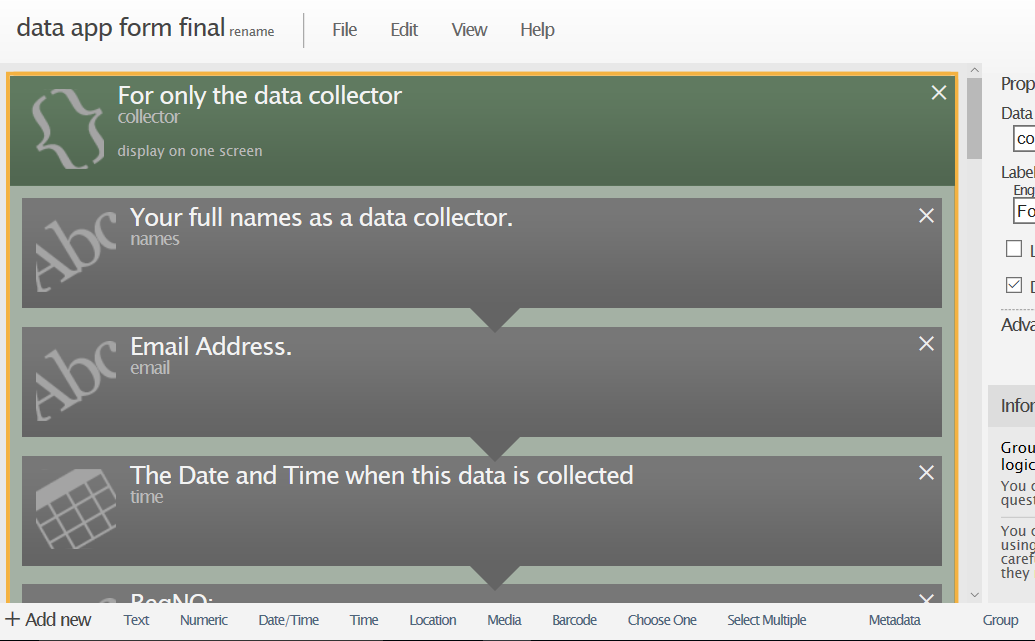
\includegraphics[width=6cm,height=8cm]{Capture}
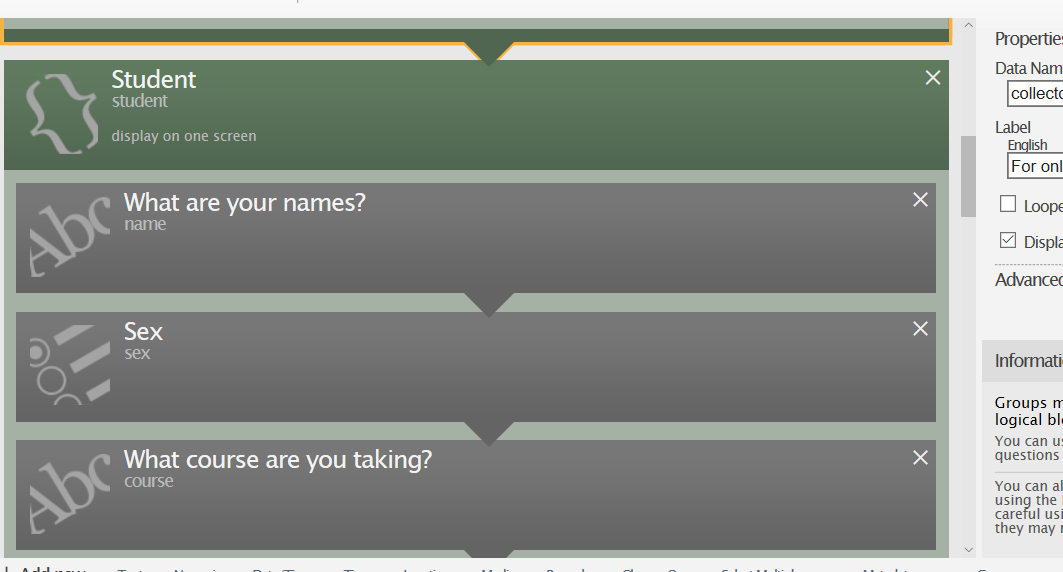
\includegraphics[width=6cm,height=8cm]{Capture1}
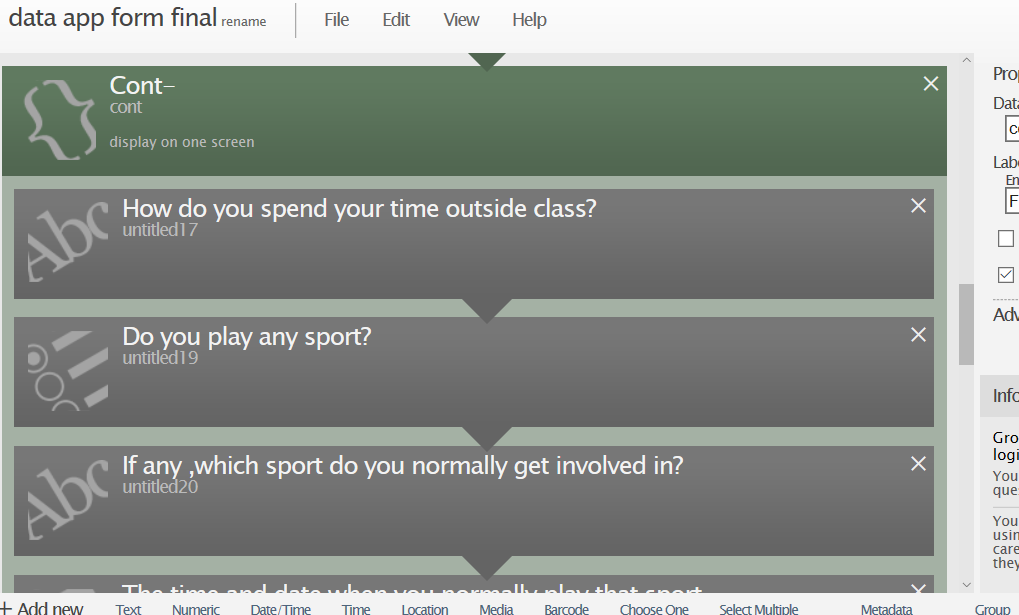
\includegraphics[width=6cm,height=8cm]{Capture2}

\includegraphics[width=6cm,height=8cm]{Capture3}
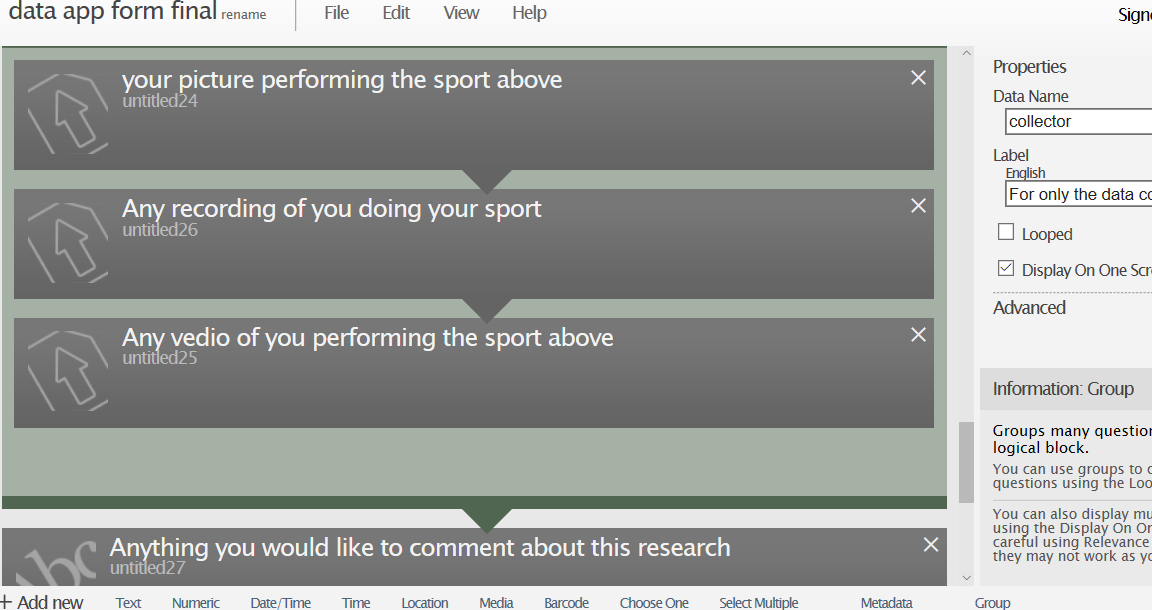
\includegraphics[width=6cm,height=8cm]{Capture4}
 
\section{Conclusions and Policy Implications.}
Physical inactivity among youth is an important public health issue and efforts to increase physical activity are sorely needed. Several national organizations, including the Institute of Medicine and the U.S. Department of Health and Human Services, have promoted sports participation as a means to increase physical activity levels.Both organizations emphasize the need to increase support for intramural sports to help provide opportunities for all students to participate in sports, regardless of skill level. The low levels of participation in intramural sports documented in this study suggest an opportunity to increase the availability and acceptability of such programs.The number of students participating in sports also can be increased by implementing a no-cut policy for interscholastic sports, whereby no students are eliminated from participation based on factors such as their skill level. 


\section{References}{
\begin{thebibliography}{1}
\bibitem{}{National Association for Sport and Physical Education. Cocurricular physical activity and sport programs for university students [Position paper]. Reston, VA: National }
\bibitem{}{Strong WB, Malina RM, Blimkie CJR, et al. Evidence based physical activity for school-age youth. J Pediatr.2005;146(6):732-737.}
\bibitem{}{National Federation of State university Associations (2011). Participation Survey, 1971�2011.Indianapolis, IN: National Federation of State university
Associations}

}


 
\end{document}


